\chapter{Overview}\label{sec:overview}

\section{Workflow Overview}

\cxoneflow has origins in CxFlow for the CxSAST product, which is the predecessor to Checkmarx One.  CxFlow
had a variety of functions and deployment options related to orchestrating scans in CxSAST and sending
result feedback to issue trackers.  \cxoneflow will also orchestrate scans but is adaptated to the
concepts of CheckmarxOne.

The \cxoneflow logic for how scans are orchestrated is very similar to that of CxFlow.  The basic
logic flow is that scans are executed when:

\begin{itemize}
    \item If a Push is made to a repository's protected branch, that protected branch is scanned.
    \item If a Pull Request is opened that targets a protected branch, a scan is performed on
    the source branch.
    \item If a Push is made to a branch that is the source of an open Pull Request that targets
    a protected branch, that branch is scanned.
\end{itemize}


\cxoneflow follows this workflow logic upon the receipt of a webhook event payload generated by the SCM.
The code from the repository to be scanned is cloned by \cxoneflow, collected into a zip file, then submitted
for a scan to CheckmarxOne.  When the scan is submitted, the cloned code is deleted.


\section{Deployment Overview}

The method of deployment for \cxoneflow is intended to integrate scanning of all enterprise repositories
with a minimal amount of configuration.  The best method for deployment is to configure source control web
hooks where they will emit events for the largest possible number of repositories.  In many source control
systems, this can be done at a global or organization level.  The web hooks will be configured to send events
to a \cxoneflow endpoint specific to the type of source control system.

Figure \ref{fig:cxoneflow-deployment} depicts the way \cxoneflow is deployed.  Some organizations may have
multiple source control systems of the same type or even multiple different types of source control systems.
There may be multiple Checkmarx One tenants or a combination of multi-tenant and single-tenant Checkmarx One
deployments.  The \cxoneflow configuration allows each endpoint to be configured such that it orchestrates
scans in the correct Checkmarx One instance for the source of the web hook event.

\begin{figure}[h]
    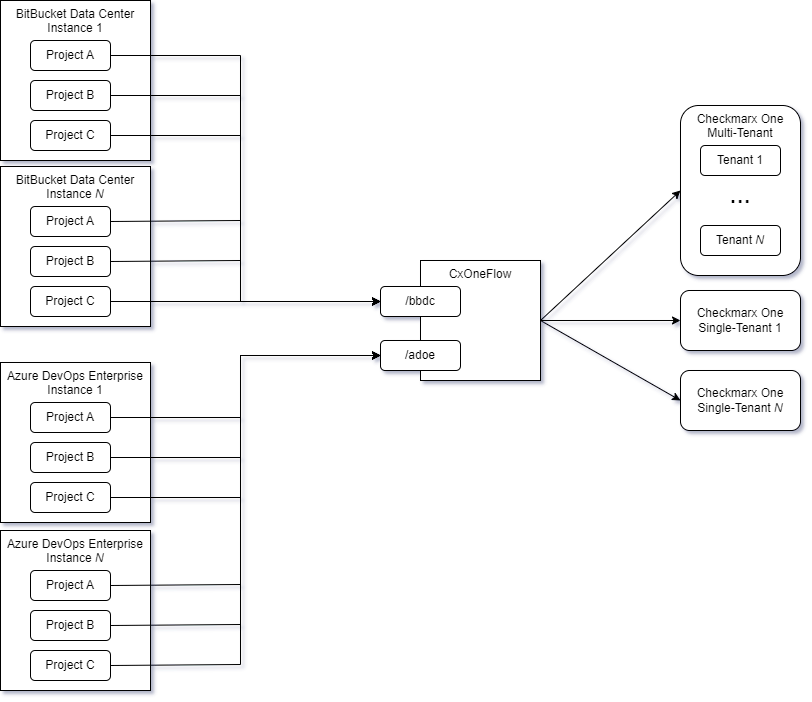
\includegraphics[width=\textwidth]{graphics/cxoneflow-deployment.png}
    \caption{\cxoneflow Deployment Diagram}
    \label{fig:cxoneflow-deployment}
\end{figure}

